
\subsection{Methods of Curve Fitting(曲线拟合)}

\frame{
\frametitle{Data Linearization Method for $y=Ce^{Ax}$}
\begin{block}{}
Suppose that we are given the points $(x_1,y_1), (x_2, y_2), \ldots , (x_N, y_N)$ and want to fit an exponential curve of the form 
\begin{equation*}
y = C e^{A x}
\end{equation*}
\end{block}
\begin{itemize}
\item The first step is to take the logarithm of both sides: 
\begin{equation*}
\ln(y) = A x + \ln(C)
\end{equation*}
\item Then introduce the change of variables: 
\begin{equation*}
Y = \ln(y),  X =x, B = \ln(C) 
\end{equation*}
\item This results in a linear relation between the new variables $X$ and $Y$: 
\begin{equation*}
Y = A X + B
\end{equation*}
\end{itemize}
}

\frame{
\begin{itemize}
\item The original points $(x_k, y_k)$ in the xy-plane are transformed into the points $(X_k, Y_k) = (x_k,\ln(y_k))$ in the $XY-$plane. 
\item This process is called data linearization. 
\item Then the least-squares line (4.23) is fit to the points $\{(X_k, Y_k)\}$. 
\item The normal equations for finding $A$ and $B$ are 
\begin{equation*}
\begin{array} {l l}
\left( \sum_{k=1}^N X_k^2 \right) A + \left( \sum_{k=1}^N X_k \right) B & = \sum_{k=1}^N X_k Y_k \\ 
& \\
\left( \sum_{k=1}^N X_k \right) A + N B & =  \sum_{k=1}^N Y_k
\end{array}
\end{equation*} 
\item After $A$ and $B$ have been found, the parameter $C$ in equation (4.20) is computed:
\begin{equation*}
C = e^B
\end{equation*}
\end{itemize}
}

\frame{
\begin{block}{Example.}	
Use the data linearization method and find the exponential fit $y = C e^{Ax}$ for the five data points $(0, 1.5)$, $(1, 2.5)$, $(2, 3.5)$, $(3, 5.0)$, and $(4, 7.5)$.
\end{block}
Apply the transformation (3) to the original points and obtain
\begin{equation*}
\begin{array}{r}
\{ ( X_k , Y_k ) \} = \{ ( 0, \ln(1.5), (1, \ln(2.5)), (2, \ln(3.5)), (3, \ln(5.0)), (4, \ln(7.5)) \} \\
= \{ (0, 0.40547), (1, 0.91629), (2, 1.25276), (3, 1.60944), (4, 2.01490) \}.
\end{array}
\end{equation*}
\begin{columns}
\begin{column}{0.5\textwidth}
\begin{figure}
\begin{center}
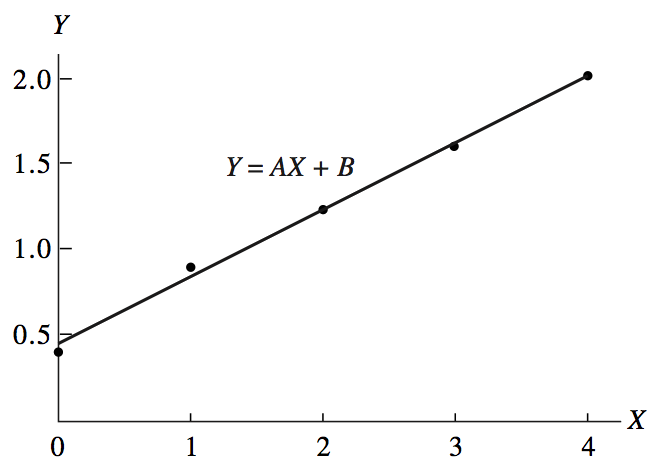
\includegraphics[width=55mm]{chap-4/fig_5-4.png}
\end{center}
\end{figure}
\end{column}
\begin{column}{0.5\textwidth}
These transformed points are shown in the left Figure  and exhibit a linearized form. 
The equation of the least-squares line $Y = A X + B$ for the points in the left Figure  is
\begin{equation*}
Y = 0.391202X + 0.457367.
\end{equation*}
\end{column}
\end{columns}
}

\frame{
\begin{itemize}
%\item Calculation of the coefficients for the normal equations in (4.24) is shown in the Table 4.4. 
\item The resulting linear system  for determining A and B is
\begin{equation*}
\begin{array}{l l}
30A + 10 B & = 16.309742 \\
10A + 5   B & = 6.198860
\end{array}
\end{equation*}
%\begin{figure}
%\begin{center}
%\includegraphics[width=50mm]{fig/ch-4/eq_4-28.png}
%\end{center}
%\end{figure}
\item The solution is $A = 0.3912023$ and $B = 0.457367$. 
\item Then $C$ is obtained with the calculation $C = e^{0.457367} = 1.579910$, and these values for $A$ and $C$ are substituted into equation (4.20) to obtain the exponential fit. 
\begin{equation*}
y = 1.579910e^{0.3912023x} \ \ \ \ \	(fit \ by \  data \  linearization).
\end{equation*}
\end{itemize}
\begin{columns}
\begin{column}{0.5\textwidth}
\begin{figure}
\begin{center}
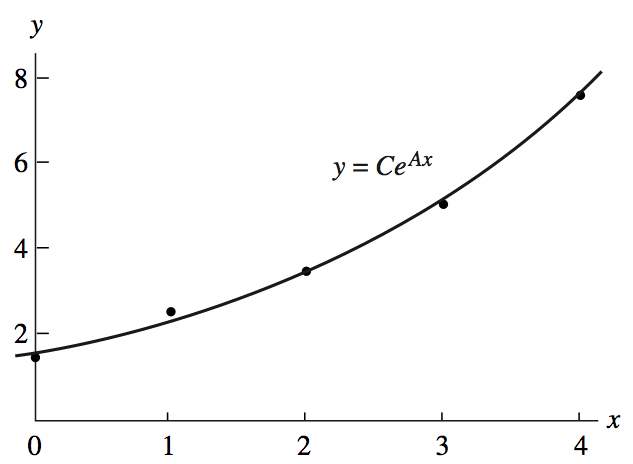
\includegraphics[width=40mm]{chap-4/fig_5-5.png}
\end{center}
\end{figure}
\end{column}
\begin{column}{0.5\textwidth}
\begin{figure}
\begin{center}
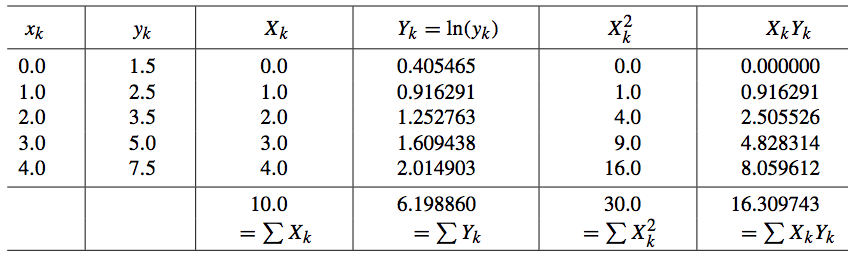
\includegraphics[width=60mm]{chap-4/tab_5-4.png}
\end{center}
\end{figure}
\end{column}
\end{columns}
}

\frame{
\frametitle{Nonlinear Least-Squares Method for $y= Ce^{Ax}$}
Suppose that we are given the points $(x_1, y_1), (x_2, y_2), \ldots, (x_N, y_N)$ and want to fit an exponential curve:
\begin{equation*}
y = C e^{A x}
\end{equation*}
The nonlinear least-squares procedure requires that we find a minimum of 
\begin{equation*}
E(A, C) = \sum_{k =1}^N \left(  C e^{A x_k} - y_k \right)^2
\end{equation*}
The partial derivatives of $E(A, C)$ with respect to $A$ and $C$ are
\begin{equation*}
\frac{\partial E}{\partial A} = 2 \sum_{k=1}^N (C e^{A x_k} - y_k)(C x_k e^{A x_k})
\end{equation*}
and
\begin{equation*}
\frac{\partial E}{\partial C} = 2 \sum_{k=1}^N (C e^{A x_k} - y_k)(e^{A x_k})
\end{equation*}
}

\frame{
When the partial derivatives in (4.32) and (4.33) are set equal to zero and then simplified, the resulting normal equations are 
\begin{equation*}
\begin{array}{l l}
C \sum_{k=1}^N x_k e^{2 A x_k} - \sum_{k=1}^N x_k y_k e^{A x_k} & = 0 \\
& \\
C \sum_{k=1}^N e^{A x_k} - \sum_{k=1}^N y_k e^{A x_k} & = 0
\end{array}
\end{equation*}
\begin{block}{}
\begin{itemize}
\item The equations in (4.34) are nonlinear in the unknowns A and C and can be solved using Newton's method. 
 This is a time-consuming computation and the iteration involved requires good starting values for $A$ and $C$. 
\item Many software packages have a built-in minimization subroutine for functions of several variables that can be used to minimize $E(A, C)$ directly.
For example, the Neider-Mead simplex algorithm can be used to minimize (4.31) directly and bypass the need for equations (4.32) through (4.34). 
\end{itemize}
\end{block}
}

\frame{
\begin{block}{Example.}
Use the least-squares method and determine the exponential fit $y = Ce^{Ax}$ for the five data points $(0, 1.5)$, $(1, 2.5)$, $(2, 3.5)$, $(3, 5.0)$, and $(4, 7.5)$.
\end{block}
First, we define $E(A, C)$ as an M-file in MATLAB.
\begin{equation*}
E(A,C)  = (C−1.5)^2 +(Ce^A −2.5)^2 +(Ce^{2A} −3.5)^2 + (Ce^{3A} − 5.0)^2 + (Ce^{4A} − 7.5)^2.
\end{equation*}
%\begin{verbatim}
%function z=E(u)
%A=u(1); 
%C=u(2); 
%z=(C-1.5).^2+(C.*exp(A)-2.5).^2+(C.*exp(2*A)-3.5).^2+...
 %     (C.*exp(3*A)-5.0).^2+(C.*exp(4*A)-7.5).^2;
%\end{verbatim}
Then, use the {\Large fmins} command in MATLAB to approximate the values of $A$ and $C$ that minimize $E(A, C)$. \\
Thus the exponential fit to the five data points is
\begin{equation*}
y = 1.6108995 e^{0.3835705} \ \ \ \ \ (fit \  by \  nonlinear \  least \  squares).
\end{equation*}
}

%\frame{
%\begin{figure}
%\begin{center}
%\includegraphics[width=110mm]{fig/ch-4/ex_4-5.png}
%\end{center}
%\end{figure}
%}

\frame{
\begin{columns}
\begin{column}{0.5\textwidth}
\begin{figure}
\begin{center}
%\includegraphics[width=50mm]{fig/ch-4/tab_5-5.png}
\includegraphics[width=50mm]{chap-4/tab_5-5.png}
\end{center}
\end{figure}
\end{column}
\begin{column}{0.5\textwidth}
\begin{figure}
\begin{center}
%\includegraphics[width=50mm]{fig/ch-4/fig_5-6.png}
\includegraphics[width=50mm]{chap-4/fig_5-6.png}
\end{center}
\end{figure}
\end{column}
\end{columns}
\begin{itemize}
\item A comparison of the solutions using data linearization and nonlinear least squares is given in the above Table . 
\item There is a slight difference in the coefficients. For the purpose of interpolation  it can be seen that the approximations differ by no more than $2\%$ over the interval $[0,4]$ . 
\item If there is a normal distribution of the errors in the data, the above equation is usually the preferred choice. 
\item When extrapolation is made beyond the range of the data, the two solutions will diverge and the discrepancy increases to about $6\%$ when $x = 10$. 
\end{itemize}
}

\frame{
\frametitle{ Transformations for Data Linearization}
\begin{itemize}
\item The technique of data linearization has been used by scientists to fit curves such as $y = Ce^{(Ax)}$, $y = A\ln(x) + B$, and $y = A/x + B$. 
\vspace{0.3cm}
\item Once the curve has been chosen, a suitable transformation of the variables must be found so that a linear relation is obtained. 
\vspace{0.3cm}
 For example, the reader can verify that $y = D/(x + C)$ is transformed into a linear problem $Y = AX + B$ by using the change of variables (and constants) $X = xy$, $Y = y$, $C = -1/A$, and $D = -B/A$. 
\vspace{0.3cm}
\item Graphs of several cases ofthe possibilities for the curves are shown in Figure 4.7, and other useful transformations are given in Table 4.6. 
\end{itemize}
}

\frame{
\begin{figure}
\begin{center}
%\includegraphics[width=110mm]{fig/ch-4/fig_4-7_1.png}
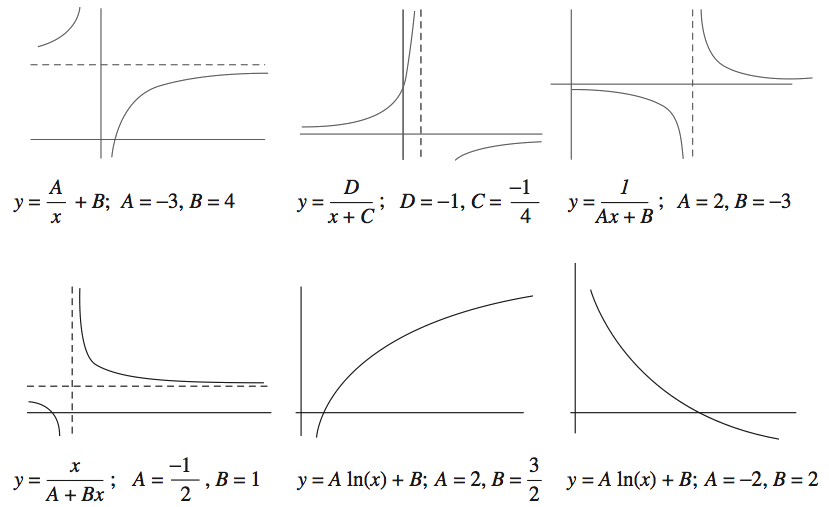
\includegraphics[width=110mm]{chap-4/fig_5-7.png}
\end{center}
\end{figure}
}

\frame{
\begin{figure}
\begin{center}
%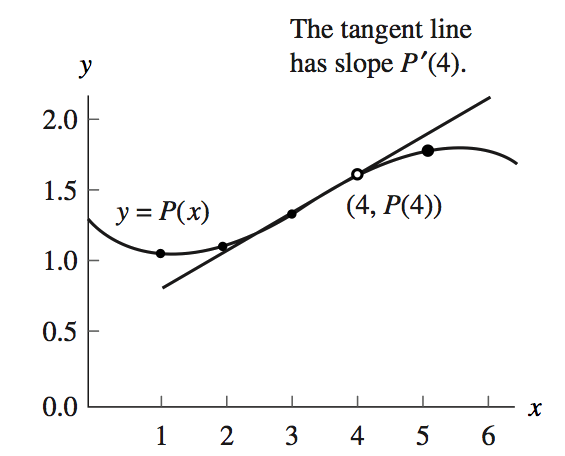
\includegraphics[width=110mm]{fig/ch-4/fig_4-7_2.png}
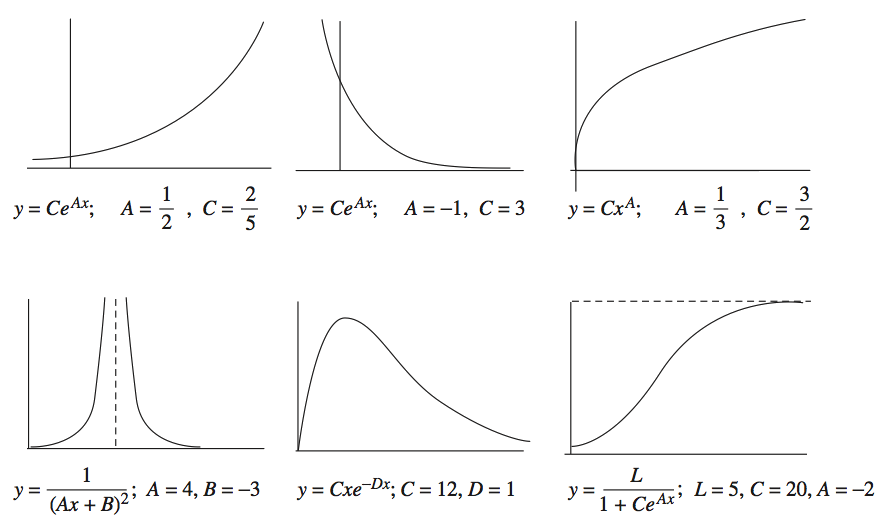
\includegraphics[width=110mm]{chap-4/fig_5-7_2.png}
\end{center}
\end{figure}
}

\frame{
\begin{figure}
\begin{center}
%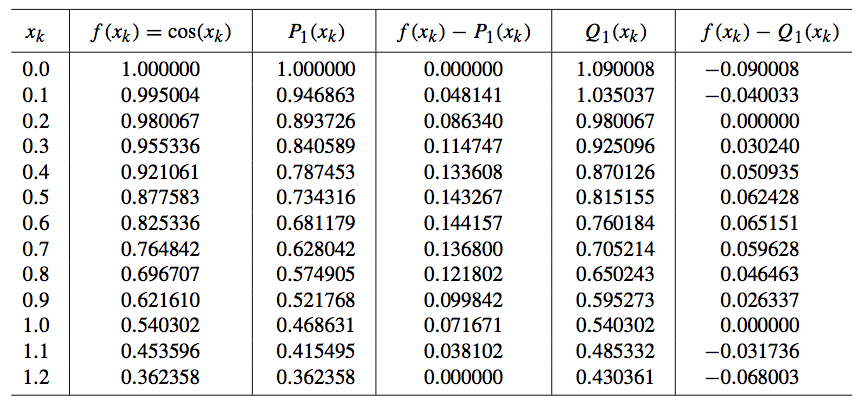
\includegraphics[width=110mm]{fig/ch-4/tab_4-6.png}
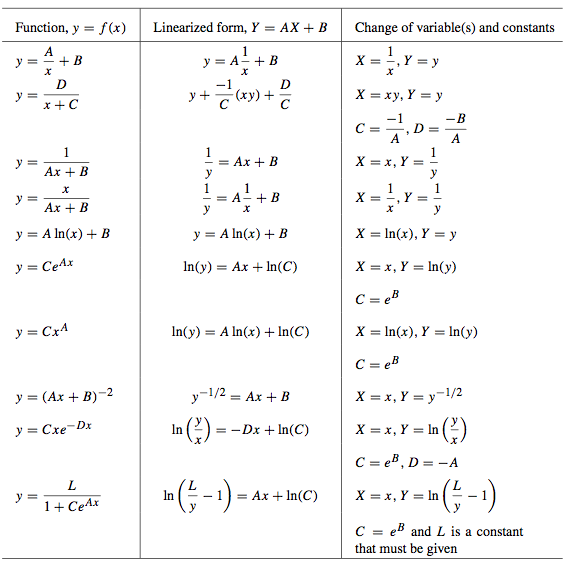
\includegraphics[width=80mm]{chap-4/tab_5-6.png}
\end{center}
\end{figure}
}

\frame{
\frametitle{Linear Least Squares}
\framesubtitle{线性最小二乘}
\begin{block}{The linear least-squares problem is stated as follows.} 
Suppose that $N$ data points $\{(x_k,y_k)\}$ and a set of $M$ linear independent functions $\{ f_j (x) \}$ are given.
\vspace{0.3cm} 
We want to find $M$ coefficients $\{ c_j \}$ so that the function $f (x)$ given by the linear combination 
\begin{equation*}
f(x) = \sum_{j=1}^{M} c_j f_j (x)
\end{equation*}
%\begin{figure}
%\begin{center}
%\includegraphics[width=70mm]{fig/ch-4/eq_4-37.png}
%\end{center}
%\end{figure}
will minimize the sum of the squares of the errors:
\begin{equation*}
E(c_1, c_2, \ldots, c_M) = \sum_{k=1}^N \left( f(x_k) - y_k\right)^2 = \sum_{k=1}^N \left( \left( \sum_{j=1}^M c_j f_j(x_k) \right) - y_k \right)^2
\end{equation*}
%\begin{figure}
%\begin{center}
%\includegraphics[width=90mm]{fig/ch-4/eq_4-38.png}
%\end{center}
%\end{figure}
\end{block}
}

\frame{
\begin{block}{}
For $E$ to be minimized it is necessary that each partial derivative be zero (i.e., $\partial E/ \partial C_i = 0$ for $i = 1, 2, \ldots , M$), and this results in the system of equations 
\begin{equation*}
\sum_{k=1}^N\left( \left( \sum_{j=1}^M c_j f_j (x_k) \right) - y_k \right) (f_i(x_k)) = 0
 \ \ \ for \ \ i = 1, 2, \ldots, M
\end{equation*}
%\begin{figure}
%\begin{center}
%\includegraphics[width=90mm]{fig/ch-4/eq_4-39.png}
%\end{center}
%\end{figure}
Interchanging the order of the summations in (4.39) will produce an $M \times M$ system of linear equations where the unknowns are the coefficients $\{ c_j \}$. They are called the normal equations:
\begin{equation*}
\sum_{j=1}^M \left( \sum_{k=1}^N f_i(x_k) f_j(x_k) \right) c_j = \sum_{k=1}^N f_i(x_k) y_k
\ \ \ for \ \ i = 1, 2, \ldots, M
\end{equation*}
%\begin{figure}
%\begin{center}
%\includegraphics[width=90mm]{fig/ch-4/eq_4-40.png}
%\end{center}
%\end{figure}
\end{block}
}

\frame{
\frametitle{Matrix Formulation}
Although (4.40) is easily recognized as a system of $M$ linear equations in $M$ unknowns, one must be clever so that wasted computations are not performed when writing the system in matrix notation.  \\
The key is to write down the matrices $F$ and $F'$ as follows:
\begin{equation*}
\begin{array}{c c}
F  = & 
\left[ 
\begin{array}{c c c c}
f_1(x_1) & f_2(x_1) & \cdots & f_M(x_1) \\
f_1(x_2) & f_2(x_2) & \cdots & f_M(x_2) \\
f_1(x_3) & f_2(x_3) & \cdots & f_M(x_3) \\
\vdots   & \vdots   &  \vdots & \vdots \\
f_1(x_N) & f_2(x_N) & \cdots & f_M(x_N) \\
\end{array}
\right]\\
F' = &
\left[ 
\begin{array}{c c c c c}
f_1(x_1) & f_1(x_2) & f_1(x_3) & \cdots & f_1(x_N) \\
f_2(x_1) & f_2(x_2) & f_2(x_3) & \cdots & f_2(x_N) \\
\vdots   & \vdots   &  \vdots   & \vdots & \vdots \\
f_M(x_1) & f_M(x_2) &f_M(x_3) & \cdots & f_M(x_N) \\
\end{array}
\right]
\end{array}
\end{equation*}
%\begin{figure}
%\begin{center}
%\includegraphics[width=60mm]{fig/ch-4/eq_4-41_1.png}
%\end{center}
%\end{figure}
}

\frame{
Consider the product of $F'$ and the column matrix $Y$: 
\begin{equation*}
F' Y = 
\left[ 
\begin{array}{c c c c c}
f_1(x_1) & f_1(x_2) & f_1(x_3) & \cdots & f_1(x_N) \\
f_2(x_1) & f_2(x_2) & f_2(x_3) & \cdots & f_2(x_N) \\
\vdots   & \vdots   &  \vdots   & \vdots & \vdots \\
f_M(x_1) & f_M(x_2) &f_M(x_3) & \cdots & f_M(x_N) \\
\end{array}
\right]
\left[
\begin{array}{c}
y_1 \\
y_2 \\
\vdots \\
y_N
\end{array}
\right]
\end{equation*}
%\begin{figure}
%\begin{center}
%\includegraphics[width=90mm]{fig/ch-4/eq_4-41_2.png}
%\end{center}
%\end{figure}
The element in the $i-$th row of the product $F'$  $Y$ in (4.41) is the same as the ith element in the column matrix in equation (4.40); 
that is, 
\begin{equation*}
\sum_{k=1}^N f_i(x_k) y_k = row_i F' \cdot \left[ y_1 \ y_2 \ \cdots y_N \right]
\end{equation*}
%\begin{figure}
%\begin{center}
%\includegraphics[width=90mm]{fig/ch-4/eq_4-42_1.png}
%\end{center}
%\end{figure}
}

\frame{
Now consider the product $F'$ $Y$, which is an $M \times M$ matrix: 
\begin{equation*}
\begin{array}{l}
F' F = \\
\left[ 
\begin{array}{c c c c c}
f_1(x_1) & f_1(x_2) & f_1(x_3) & \cdots & f_1(x_N) \\
f_2(x_1) & f_2(x_2) & f_2(x_3) & \cdots & f_2(x_N) \\
\vdots   & \vdots   &  \vdots   & \vdots & \vdots \\
f_M(x_1) & f_M(x_2) &f_M(x_3) & \cdots & f_M(x_N) \\
\end{array}
\right]
\left[ 
\begin{array}{c c c c}
f_1(x_1) & f_2(x_1) & \cdots & f_M(x_1) \\
f_1(x_2) & f_2(x_2) & \cdots & f_M(x_2) \\
f_1(x_3) & f_2(x_3) & \cdots & f_M(x_3) \\
\vdots   & \vdots   &  \vdots & \vdots \\
f_1(x_N) & f_2(x_N) & \cdots & f_M(x_N) \\
\end{array}
\right]
\end{array}
\end{equation*}
}

\frame{
The element in the $i-$th row and $j-$th column of $F' F$ is the coefficient of $c_j$ in the $i-$th row in equation (4.40); that is, 
\begin{equation*}
\sum_{k=1}^N f_i(x_k)  f_j(x_k) = f_i (x_1) f_j(x_1) + f_i(x_2) f_j(x_2) + \cdots + f_i(x_N) f_j(x_N)
\end{equation*}
When $M$ is small, a computationally efficient way to calculate the linear least-squares coefficients for (3.37) is to store the matrix $F$, compute $F' F$, and $F' Y$ and then solve the linear system
\begin{equation*}
F' F C = F' Y \ \ \ \ for \ the \ coefficient \ matrix \ C
\end{equation*}
}

\frame{
\frametitle{Polynomial Fitting}
When the foregoing method is adapted to using the functions $\{ f_j(x) = x^{j-1} \}$ and the index of summation ranges from $j = 1$ to $j = M + 1$, the function $f(x)$ will be a polynomial of degree $M$: 
\begin{equation*}
f(x) = c_1 + c_2 x + c_3 x^2 + \cdots + c_{M+1} x^M 
\end{equation*}
We now show how to find the {\Large least-squares parabola}, and the extension to a polynomial of higher degree is easily made and is left for the reader. 
}

\frame{
\begin{block}{Theorem 5.3 (Least-Squares Parabola).}
Suppose that $\{(x_k , y_k )\}^N_{k=1}$ are $N$ points, where the abscissas are distinct. 
The coefficients of the least-squares parabola
\begin{equation*}
y = f(x) = A x^2 + B x + C
\end{equation*}
are the solution values $A$, $B$, and $C$ of the linear system
\begin{equation*}
\begin{array}{l l}
\left( \sum_{k=1}^N x_k^4 \right) A + \left( \sum_{k=1}^N x_k^3 \right) B + \left( \sum_{k=1}^N x_k^2\right) C& = \sum_{k=1}^N y_k x_k^2\\
& \\
\left( \sum_{k=1}^N x_k^3 \right) A + \left( \sum_{k=1}^N x_k^2 \right) B + \left( \sum_{k=1}^N x_k \right)  C & = \sum_{k=1}^N y_k x_k \\
& \\
\left( \sum_{k=1}^N x_k^2 \right) A + \left( \sum_{k=1}^N x_k \right) B + N C & = \sum_{k=1}^N y_k 
\end{array}
\end{equation*}
\end{block}
}

%\frame{
%\begin{figure}
%\begin{center}
%\includegraphics[width=110mm]{fig/ch-4/theorem_4-3.png}
%\end{center}
%\end{figure}
%}

\frame{
\frametitle{Proof of Theorem 4.3.}
\begin{block}{}
The coefficients $A$, $B$, and $C$ will minimize the quantity:
\begin{equation*}
E (A, B, C) = \sum_{k=1}^N \left( A x_k^2 + B x_k + C - y_k \right)^2
\end{equation*}
The partial derivatives  $\partial E / \partial A$, $\partial E / \partial B$, and $\partial E / \partial C$ must all be zero.
\begin{equation*}
\begin{array}{c c c}
0 = & \frac{\partial E(A, B, C)}{\partial A} = & 2 \sum_{k=1}^N \left( A x_k^2 + B x_k + C - y_k \right)^1 (x_k^2) \\
& & \\
0 = & \frac{\partial E(A, B, C)}{\partial B} = & 2 \sum_{k=1}^N \left( A x_k^2 + B x_k + C - y_k \right)^1 (x_k)  \\
& & \\
0 = & \frac{\partial E(A, B, C)}{\partial C} = & 2 \sum_{k=1}^N \left( A x_k^2 + B x_k + C - y_k \right)^1 (1)
\end{array}
\end{equation*}
%\begin{figure}
%\begin{center}
%\includegraphics[width=110mm]{fig/ch-4/theorem_4-3_proof.png}
%\end{center}
%\end{figure}
\end{block}
%Using the distributive property of addition, we can move the values $A$, $B$, and $C$ outside the summations in (4.49) to obtain the normal equations that are given in the Theorem 5.3. %(4.47)
}

\frame{
\begin{block}{Example 4.6.}
Find the least-squares parabola for the four points $(−3, 3)$, $(0, 1)$, $(2, 1)$, and $(4, 3)$.
\end{block}
The entries in the following Table  are used to compute the summations required in the linear system (28).
The linear system (28) for finding $A$, $B$, and $C$ becomes
\begin{equation*}
\begin{array}{r r r r}
353A + & 45B + & 29C = & 79 \\
 & & &\\
45A + & 29B + & 3C = & 5  \\
 & & &\\
29A + & 3B + & 4C = & 8.
\end{array}
\end{equation*}
}

\frame{
The solution to the linear system is $A = 585/3278$, $B = −631/3278$, and $C = 1394/1639$, and the desired parabola is (see Figure 5.8)
\begin{equation*}
y = \frac{585}{3278}  x^2 − \frac{631}{3278} x + \frac{1394}{1639} = 0.178462 x^2 − 0.192495 x + 0.850519.
\end{equation*}
\begin{columns}
\begin{column}{0.5\textwidth}
\begin{figure}
\begin{center}
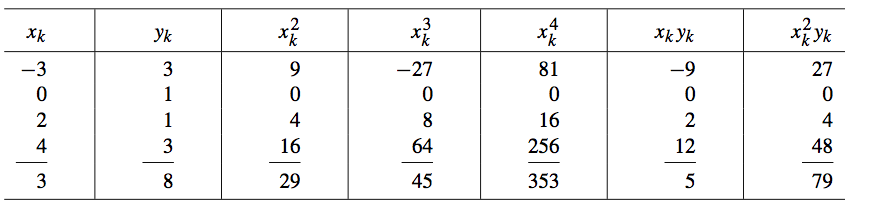
\includegraphics[width=70mm]{chap-4/tab_5-7.png}
\end{center}
\end{figure}
\end{column}
\begin{column}{0.5\textwidth}
\begin{figure}
\begin{center}
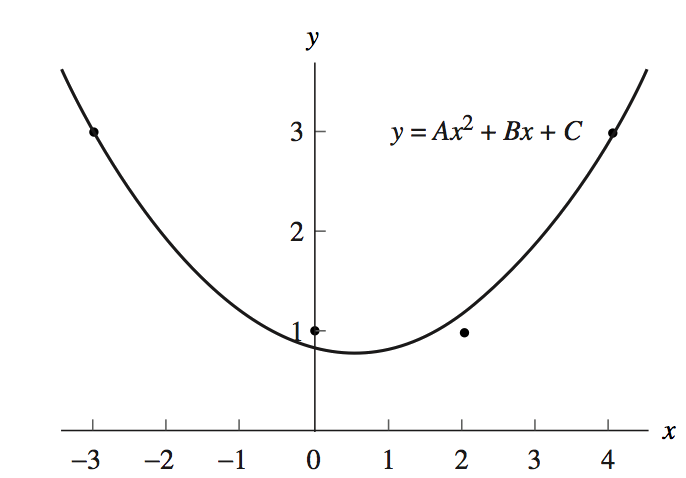
\includegraphics[width=60mm]{chap-4/fig_5-8.png}
\end{center}
\end{figure}
\end{column}
\end{columns}
}

%\frame{
%\begin{figure}
%\begin{center}
%\includegraphics[width=110mm]{fig/ch-4/ex_4-6.png}
%\end{center}
%\end{figure}
%\begin{columns}
%\begin{column}{0.5\textwidth}
%\begin{figure}
%\begin{center}
%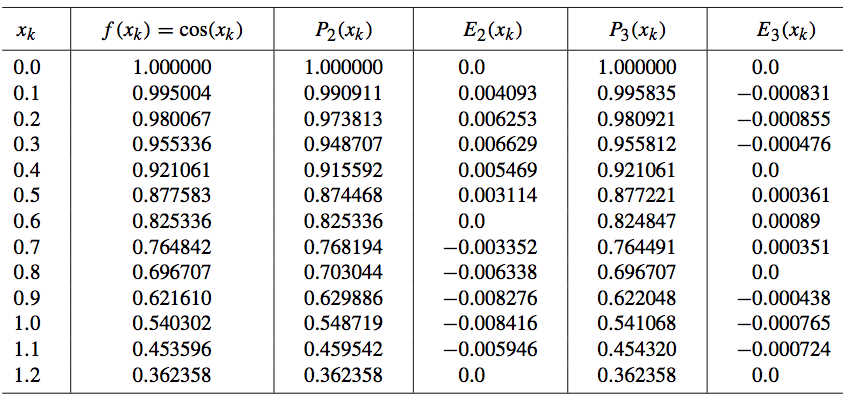
\includegraphics[width=60mm]{fig/ch-4/tab_4-7.png}
%\end{center}
%\end{figure}
%\end{column}
%\begin{column}{0.5\textwidth}
%\begin{figure}
%\begin{center}
%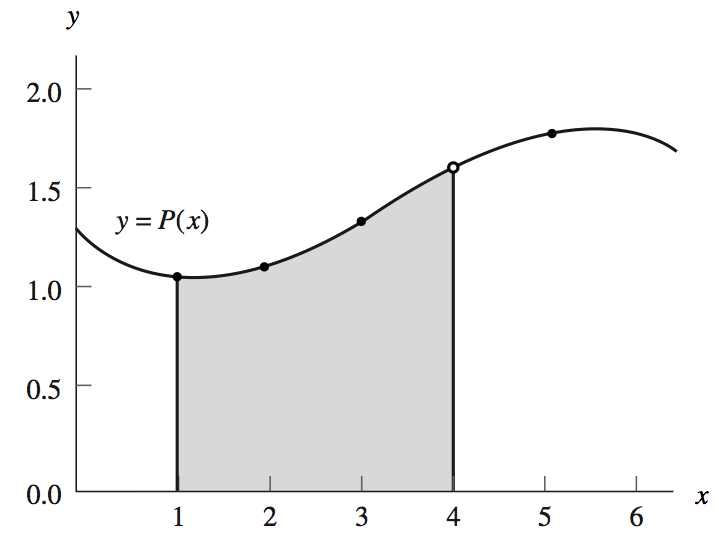
\includegraphics[width=50mm]{fig/ch-4/fig_4-8.png}
%\end{center}
%\end{figure}
%\end{column}
%\end{columns}
%}

\frame{
\frametitle{Polynomial Wiggle}
\framesubtitle{多项式震动}
\begin{itemize}
\item It is tempting to use a least-squares polynomial to fit data that are nonlinear. 
\vspace{0.5cm}
\item But if the data do not exhibit a polynomial nature, the resulting curve may exhibit large oscillations\footnote{震动,抖动}. 
 This phenomenon, called {\Large polynomial wiggle}, becomes more pronounced with higher-degree polynomials. 
\end{itemize}
\vspace{0.5cm}
\begin{block}{}
{\Large For this reason we seldom use a polynomial of degree 6 or above unless it is known that the true function we are working with is a polynomial. }
\end{block}
}

\frame{
\begin{block}{Example}
let $f(x) = 1.44/x^2 + 0.24x$ be used to generate the six data points $(0.25,23.1)$, $(1.0,1.68)$, $(1.5,1.0)$, $(2.0,0.84)$, $(2.4,0.826)$, and $(5.0,1.2576)$. 
\end{block}
The result of curve fitting with the least-squares polynomials 
\begin{equation*}
\begin{array}{l}
P_2(x) = 22.93 − 16.96 x + 2.553 x^2, \\
P_3(x) = 33.04 − 46.51 x + 19.51 x^2 − 2.296 x^3,  \\
P_4(x) = 39.92 − 80.93 x + 58.39 x^2 − 17.15 x^3 + 1.680 x^4, \\
P_5(x) = 46.02 − 118.1 x + 119.4 x^2 − 57.51 x^3 + 13.03 x^4 − 1.085 x^5
\end{array}
\end{equation*}
}

\frame{
%The following program uses the matrix $F$ with entries $f_j(x) = x_k^{j-1}$ from equation (4.37). 
\begin{figure}
\begin{center}
%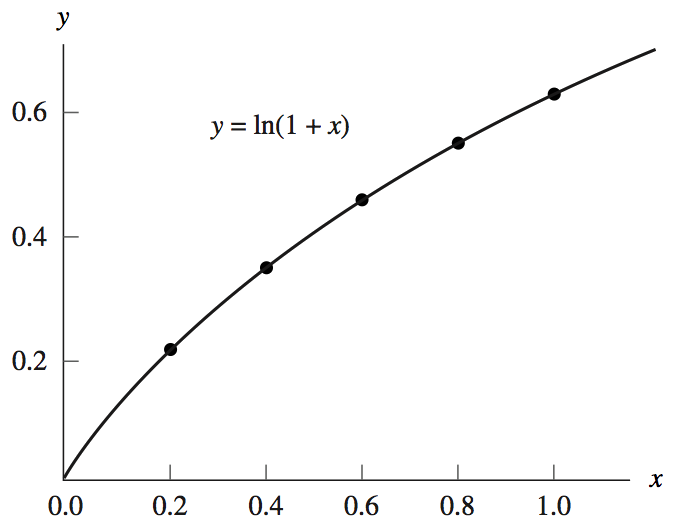
\includegraphics[width=100mm]{fig/ch-4/fig_4-9.png}
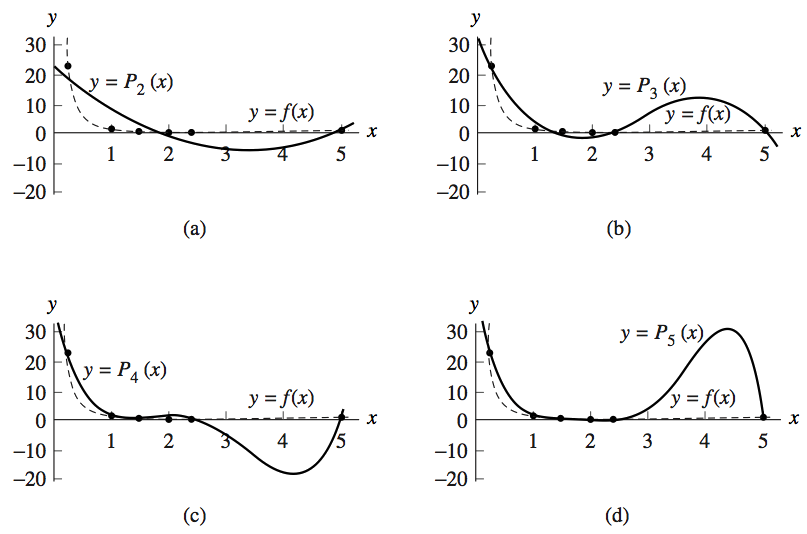
\includegraphics[width=100mm]{chap-4/fig_5-9.png}
\end{center}
\end{figure}
\begin{block}{}
Notice that $P_3(x)$, $P_4(x)$, and $P_5(x)$ exhibit a large wiggle in the interval $[2,5]$. 
%Even though $P_5(x)$ goes through the six points, it produces the worst fit. 
%If we must fit a polynomial to these data, $P_2(x)$ should be the choice. 
\end{block}
}

%\frame{
%\begin{figure}
%\begin{center}
%\includegraphics[width=110mm]{fig/ch-4/prog_4-2.png}
%\end{center}
%\end{figure}
%}

